\subsection{Hinzufügen der Stationen}
\label{sub:hinzufügen_der_stationen}
  Nachdem die Polyline auf die Karte gebracht wurde, werden die Stationen des Trips benötigt (Abbildung \ref{fig:prozess/add_stations}). Diese beinhalten für die Animation essentielle Daten wie zum Beispiel Abfahrts- und Ankunftszeit eines Vehicles. Die genaue SQL-Abfrage dafür soll an dieser Stelle der Einfachheit wegen, ausgespart bleiben.

  \begin{figure}[htbp]
    \begin{center}
      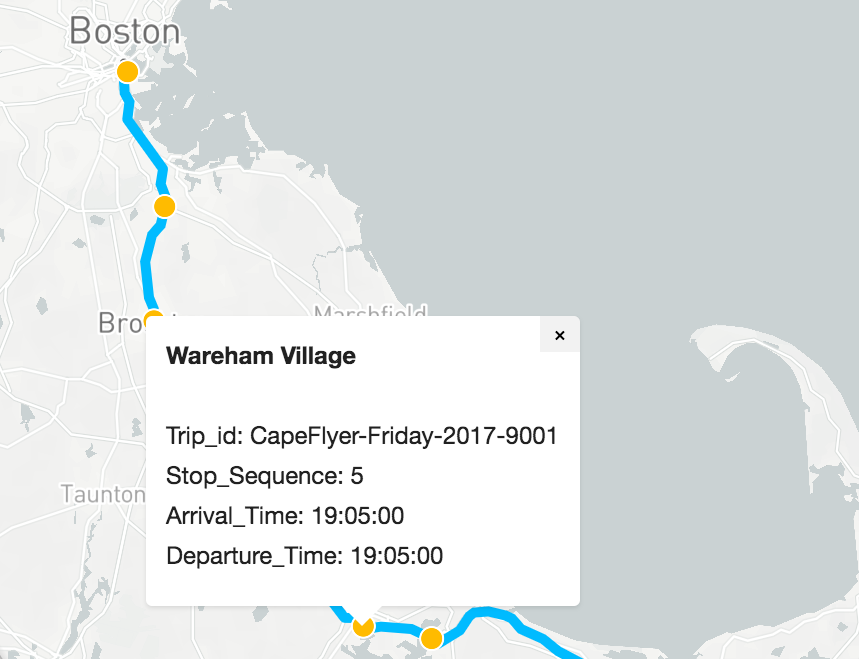
\includegraphics[width=0.5\textwidth]{prozess/add_stations}
      \caption{Hinzufügen von Stationen entlang der Polyline}
      \label{fig:prozess/add_stations}
    \end{center}
  \end{figure}

  Für die Animation der Vehicle (Abschnitt \ref{sub:animieren_eines_vehicles_durch_interpolation}) wird außerdem der Wert für die Differenz der \texttt{distance\_traveled}, also die Distanz zwischen den einzelnen Stationen, benötigt. Diese kann aus den distance\_traveled Werten der einzelnen Stationen über Subtraktion berechnet werden. Nun hat zwar das Stuttgart-VVS Feed ein distance\_traveled Feld, welches die benötigten Distanz-Informationen direkt aus der Datenbank liefert; für andere GTFS-Feeds, die getestet wurden, ist dieses Feld jedoch oftmals nicht vorhanden. Aus diesem Grund wurde ein Algorithmus entwickelt, welcher über ein sogenanntes \texttt{Station Matching} die Werte der distance\_traveled und damit die Distanz zwischen den Stationen ermitteln kann. Der Station Matching Algorithmus wird von der Applikation nur dann als Fallback-Lösung für die Berechnung verwendet, wenn das distance\_traveled Feld nicht vorhanden ist.

  \subsubsection*{Station Matching}
  \label{ssub:station_matching}
    Das Station Matching soll folgendes Problem lösen:

    \begin{figure}[htbp]
      \begin{center}
        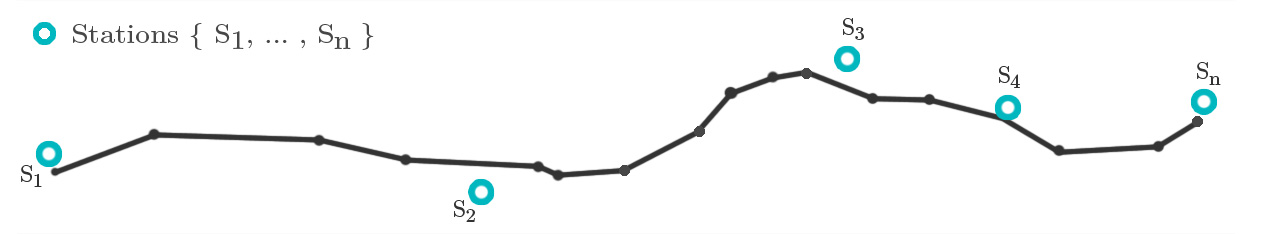
\includegraphics[width=\textwidth]{station_problem.jpg}
        \caption{Stationen liegen nicht direkt auf der Polyline}
        \label{fig:station_problem}
      \end{center}
    \end{figure}
    
    Wie in Abbildung \ref{fig:station_problem} zu sehen ist, sind die Stationen (Haltestellen oder Bahnhöfe) nicht exakt auf der Polyline, sondern ein wenig abseits positioniert, da dies auch ihrem realen Standort neben der Fahrbahn entspricht. Um nun die Distanzen zwischen den Stationen zu berechnen, legt der Algorithmus im Sinne des Matchings zunächst die Stationen auf die Polyline.  

    \begin{figure}[htbp]
      \begin{center}
        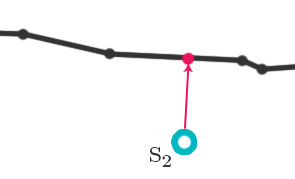
\includegraphics[width=0.25\textwidth]{find_nearest_point}
        \caption{Finde den am nächstgelegenen Punkt der Station auf der Polyline}
        \label{fig:find_nearest_point}
      \end{center}
    \end{figure}

    Nachdem der entsprechende Punkt auf der Polyline gefunden wurde, berechnet der Algorithmus die jeweiligen Wegstrecken zur ersten Station des Trips (distance\_traveled), bevor er die Werte von aufeinanderfolgenden Stationen subtrahiert.  Die Distanzen zweier Stationen $\{S_i,S_{i+1} \;|\; i \in \mathbb{N} \}$ sei $d_\triangle$. Diese kann jetzt wie folgt berechnet werden: $d_{\triangle_i} = d_{S_n} - d_{S_{n-1}}\;|\; d_S := DistanceTraveled, n \in \mathbb{N}, n \ge 2$ 
    In Listing \ref{lst:match_station} des Anhangs wird dieser Station Matching Algorithmus vorgestellt.

    \begin{figure}[htbp]
      \begin{center}
        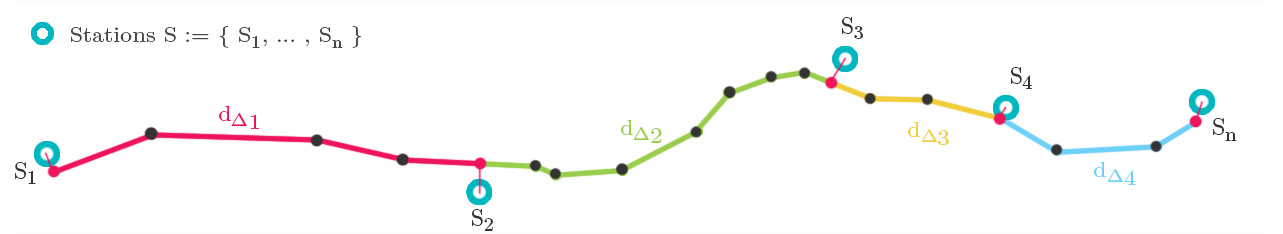
\includegraphics[width=\textwidth]{get_distances}
        \caption{Berechnen der Distanz}
        \label{fig:get_distances}
      \end{center}
    \end{figure}
    
    Abbildung \ref{fig:station_matching_comparision} stellt eine frühere Implementierung mit der nun aktuellen Version des Algorithmus gegenüber, indem die für das Matching über $n$-Trips benötigte Zeit der beiden Algorithmen verglichen wird. Um eine durchschnittliche Laufzeit zu erhalten, wurde jeder Algorithmus 10 mal mit der gleichen Anzahl an Trips ausgeführt.

    \begin{figure}[ht]
      \begin{center}
        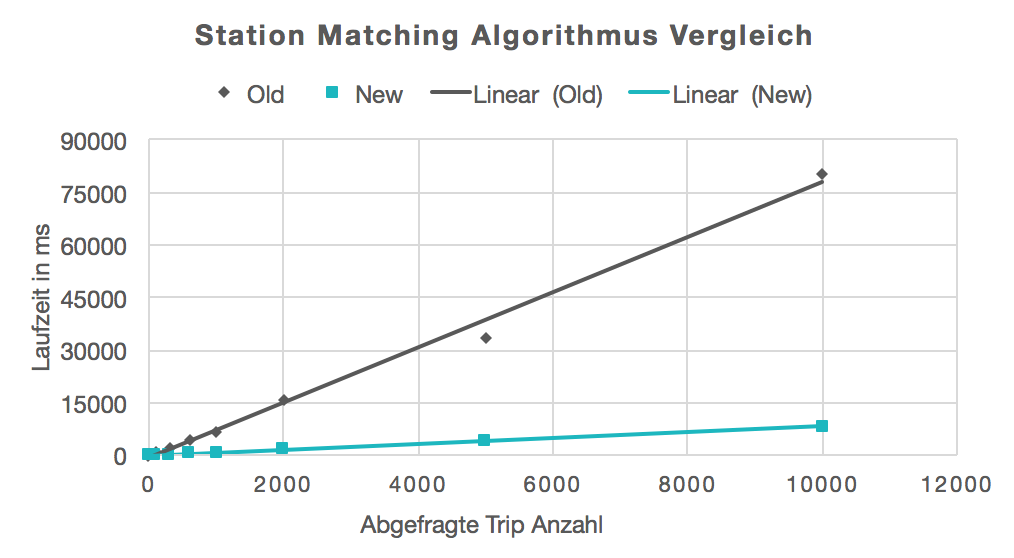
\includegraphics[width=0.7\textwidth]{station_matching_comparision}
        \caption{Vergleich der zwei Station Matching Algorithmen}
        \label{fig:station_matching_comparision}
      \end{center}
    \end{figure}

    Der alte Algorithmus war sehr simpel und beruhte darauf, die Funktion \texttt{pointOnLine} der \texttt{Turf.js} Bibliothek zu verwenden. Diese Funktion hatte den entscheidenden Nachteil, dass sie in 3 \texttt{for}-Schleifen über die gesamten Punkte der Polyline iteriert. Hinzu kommt, dass das Matching nicht nur auf eine Station, sondern auf sämtliche Stationen aus allen Trips angewendet werden muss. Das führte dazu, dass insgesamt 5 \texttt{for}-Schleifen verwendet wurden. Damit lässt sich der im Vergleich höhere Anstieg der Laufzeit bei steigender Trip Anzahl erklären. Generell ist der neue Algorithmus sehr viel schneller. Durch die Verwendung eines \texttt{R-Trees}\footnotemark und der eigenen Implementierung verschiedener Bibliotheksfunktionen (turf.lineSlice, turf.pointOnLine), konnte die Laufzeit drastisch reduziert werden (siehe Tabelle \ref{tbl:station_matching_comparison}).

    \footnotetext{Ein R-Tree (R für Rectangle) bezeichnet eine baumförmige Datenstruktur für das Speichern und Abfragen von raumbezogenen Informationen. In Verwendung ist folgende Bibliothek: \url{https://github.com/mourner/rbush}}

    \begin{longtable}{|>{\raggedright \arraybackslash}p{5.0cm}|>{\raggedright \arraybackslash}p{5.0cm}|>{\raggedright \arraybackslash}p{5.0cm}|}
    \caption{Station Matching Vergleich Old / New}\label{tbl:station_matching_comparison}\\
      \hline
      Anz. verarbeiteter Trips & Old (in ms)& New (in ms)\\
      \hline
      100    & 712   & 121  \\
      300    & 2191  & 305  \\
      600    & 4344  & 545  \\
      1.000  & 6780  & 874  \\
      2.000  & 15782 & 1700 \\
      5.000  & 33708 & 4161 \\
      10.000 & 80291 & 8279 \\
      \hline
    \end{longtable}

    Zwar wachsen beide Implementierungen lediglich linear mit steigender Trip-Anzahl, allerdings benötigt der neue Algorithmus für die Verarbeitung von $10.000$ Trips anstatt $80.29$ nur $8.28$ Sekunden.  

    Im Realbetrieb verarbeitet der Server zwischen $0 - 500$ Trips. Bei dieser Anzahl beträgt die Laufzeit des Algorithmus $\approx80ms - 400ms$. Dadurch kann argumentiert werden, dass der Algorithmus gerade noch schnell genug für eine Webanwendung arbeitet. Auch größere Anzahlen an Trips wären noch in akzeptabler Geschwindigkeit berechenbar. So können $1000$ Trips immer noch in unter einer Sekunde berechnet werden. Allerdings wäre es bei einer größeren Anzahl an Trips ein falscher Ansatz, diese bei jeder Serveranfrage neu zu kalkulieren.

    Besser wäre es, einmalig das Matching für alle Trips eines GTFS Feeds durchzuführen und die Ergebnisse persistent in der Datenbank abzuspeichern. Dies könnte beispielsweise gleich beim Importieren der Daten in die Datenbank geschehen. Dadurch könnte die Berechnung komplett eingespart werden. 
    Da für das Stuttgart-VVS Feed glücklicherweise die zurückgelegte Distanz bis zu einer Station bereits zur Verfügung steht, muss nur noch die Distanz zwischen den Stationen ($d\triangle$) berechnet werden. Dies geschieht nach dem selben Prinzip wie in der oben genannten Subtraktions-Formel. Diese Berechnung ist trivial und erfolgt bei $10.000$ Trips in unter 15 Millisekunden.

  % subsubsection station_matching (end)
% subsection hinzufügen_der_stationen (end)